\chapter{Experimental Work}
\label{chap:experimental_work}

\improvement[inline]{Put here things from intro and modify}{Start}
In this research project, a self-balancing mini-bike developed by \textbf{WHEELTEC} was utilized as the experimental platform. The primary goal of the project is to implement a data-driven State-Feedback Controller for stabilizing the bike. The mini-bike is equipped with various sensors and actuators to enable control and data acquisition.
\todo[inline]{Add Tapken's work on the same bike with simulink modelling for it.}
%% Mini-Bike Overview Section for Thesis

\subsection{Mini-Bike Structure and Components}
The mini-bike is based on the \textbf{WHEELTEC Z100 Servo Self-Balancing Bicycle} in Figure \ref{fig:minibike}. It features an STM32F103C8T6 microcontroller as the primary control unit, which integrates differenct sensors and motor control circuits to achieve stabilization. The bike has the following key components:
\begin{itemize}
	\item \textbf{Gyroscope (MPU6050)}: Provides angular velocity and acceleration data necessary for balancing the bike.
	\item \textbf{Motor and Encoder}: The rear wheel motor is driven by an H-bridge circuit (AT8236), while the encoder measures rotational speed and position, enabling closed-loop control.
	\item \textbf{Servo Motor}: Controls the steering mechanism, essential for maintaining balance during motion.
	\item \textbf{Power Supply}: Powered by a 2S lithium-ion battery, maintaining an optimal voltage range of 7 to 12 volts.
	\item \textbf{Bluetooth Module}: Allows remote control and data transmission via the MiniBalance mobile app.
\end{itemize}

\unsure[inline]{Remove structure?}
\subsection{Balancing and Control Mechanism}
The bike achieves self-balancing through controlling the steering angle. This is done through a controller computed using \textbf{Linear Quadratic Regulator (LQR)} combined with a \textbf{PID controller}. The LQR calculates optimal control inputs based on the state feedback to minimize the cost function, while the PID controller fine-tunes the steering speed by adjusting the PWM signals to the servo motor.

The system's balance is continuously monitored through the gyroscope, which provides real-time data on tilt angles and angular velocities. These values are processed by the microcontroller to compute the necessary adjustments to the rear wheel and steering servo to maintain balance.

\subsection{Data Collection and Experimental Setup}
Data from the bike can be collected using the \textbf{USART1} for transmission to a host computer and \textbf{USART3} for Bluetooth communication. The mobile application displays data such as tilt angles, angular velocity, and PWM values, allowing for parameter adjustments during testing.

\subsection{Operation and Control Interface}
The mini-bike can be operated using a mobile application that connects via Bluetooth. The app allows the user to control the bike's direction and view live data for diagnostic purposes. Additionally, a waveform display can be accessed via a PC for more detailed analysis.

\subsection{Challenges and Adjustments}
One of the challenges encountered was the adjustment of the balance midpoint, which can be fine-tuned using potentiometers located on the main board. These potentiometers adjust the balance point without needing to modify the control algorithm directly, which is particularly useful for maintaining stability under varying conditions.

In summary, the WHEELTEC mini-bike served as an experimental platform for the implementation and testing of the data-driven feedback controller, providing a practical application for a stabilisation system.

\begin{figure}
	\centering
	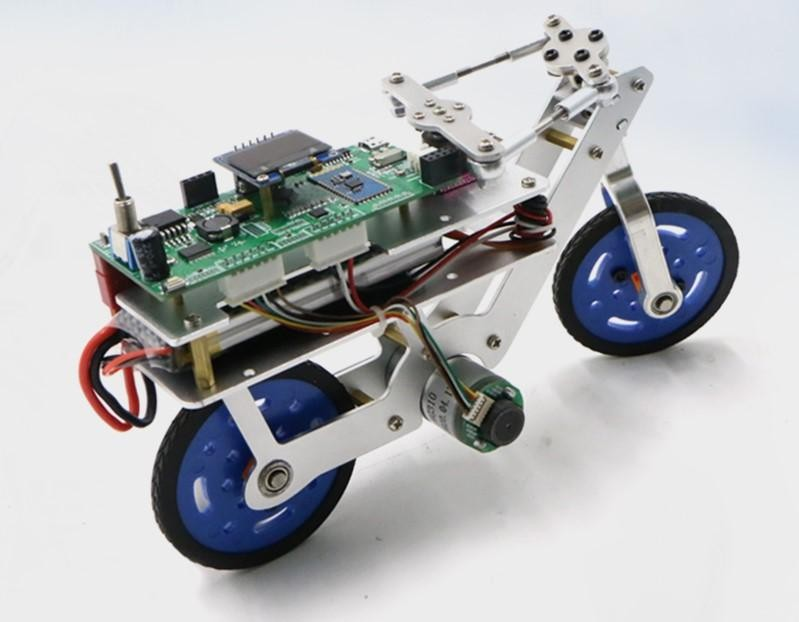
\includegraphics[width=0.7\linewidth]{figures/minibike/minibike}
	\caption{A picture for the MiniBike used in the experiments.}
	\label{fig:minibike}
\end{figure}

\improvement[inline]{Put here things from intro and modify}{End}

\section{Hardware Setup}

The experimental validation of the designed controllers was carried out using the WHEELTEC Z100 Mini-Bike platform described in Section~\ref{sec:minibike}.
The primary hardware components of the system are summarized as follows:

\begin{itemize}
	\item \textbf{Microcontroller:} STM32F103C8T6 (ARM Cortex-M3)
	\item \textbf{IMU Sensor:} MPU6050 (3-axis gyroscope and accelerometer)
	\item \textbf{Servo Motor:} WHEELTEC Z100 steering servo
	\item \textbf{Rear Wheel Motor:} DC motor with incremental encoder
	\item \textbf{Motor Driver:} AT8236 H-bridge circuit
	\item \textbf{Power Supply:} 2S lithium-ion battery (7--12 V)
	\item \textbf{Wireless Communication:} Bluetooth module (USART3)
\end{itemize}

Data acquisition and control commands were handled by the STM32 microcontroller operating at a sampling frequency of $100$~Hz.
Communication with the host computer for debugging and data logging was achieved through a UART serial interface.

\section{Software Implementation}

The control algorithms were implemented on the STM32 using C++ programming with HAL Drivers.
Key implementation steps included:
\begin{itemize}
	\item Reading IMU data (lean angle and angular velocity) via I2C communication.
	\item Processing encoder pulses to estimate forward velocity.
	\item Applying a complementary filter to estimate the lean angle more robustly.
	\item Implementing the state-feedback controller (LQR) and switching later to the Data-Driven MPC control law.
	\item Controlling the steering servo via PWM signal modulation.
	\item Logging real-time data through USART1 to a PC terminal for offline analysis.
	\item \todo{Bluetooth}
\end{itemize}

The real-time computation of the Data-Driven MPC control law involved solving a semi-definite programming (SDP) problem.
Due to computational limitations of the STM32, the SDP optimization was first performed offline, and the resulting state-feedback gain matrix was embedded into the embedded controller as a static gain.

\section{Data Collection}

Two types of data were collected during the experiments:
\begin{itemize}
	\item \textbf{Open-loop Data:} System response without feedback control to characterize the dynamics and validate the bicycle model.
	\item \textbf{Closed-loop Data:} System response under the LQR and Data-Driven MPC controllers.
\end{itemize}

The following signals were recorded:
\begin{itemize}
	\item Lean angle ($\phi$)
	\item Lean rate ($\dot{\phi}$)
	\item Steering angle ($\delta$)
	\item Control input (steering rate command)
	\item Motor encoder readings (optional)
\end{itemize}

Data was logged at a sampling rate of $100$~Hz, synchronized with control execution.

\section{Experimental Procedure}

The experimental procedure involved the following steps:
\begin{enumerate}
	\item Calibrate the IMU sensor to eliminate initial offsets.
	\item Start the bicycle with an initial forward velocity manually achieved by a push.
	\item Apply the selected controller (LQR or Data-Driven MPC).
	\item Record the system's lean angle and steering angle evolution during the stabilization process.
	\item Introduce manual disturbances by slightly perturbing the bicycle during motion.
	\item Stop the experiment after achieving stabilization or falling.
\end{enumerate}

Each experimental run was repeated multiple times to ensure reproducibility and to evaluate the robustness of the controller under different initial conditions and disturbances.

\section{Challenges Encountered}

Several practical challenges were encountered during the experimental phase:
\begin{itemize}
	\item \textbf{Sensor Noise:} The MPU6050 exhibited significant noise at low velocities, requiring careful filtering and calibration.
	\item \textbf{Timing and Delays:} Limited computational resources led to minor delays in control signal update, impacting the system's responsiveness.
	\item \textbf{Motor Saturation:} The servo motor exhibited saturation effects at high steering rates, limiting the maximum achievable control torque.
	\item \textbf{Balance Midpoint Drift:} Fine adjustments of the potentiometer on the main board were necessary to maintain correct balance points without modifying the control code.
\end{itemize}

Despite these challenges, stable experimental results were obtained, validating the effectiveness of the proposed data-driven control strategy.
